% !TeX encoding = UTF-8
% !TeX spellcheck = en_GB

\documentclass[fleqn]{scrartcl}

% Package for typography
\usepackage{microtype}
\usepackage{appendix}

% Packages for graphics and figures
\usepackage{graphicx}
\usepackage{booktabs}
\usepackage{multirow}
\usepackage{bigdelim}
\usepackage{flafter}
%\usepackage{floatrow}
\usepackage{rotating}
% https://tex.stackexchange.com/a/77945
\newsavebox\CaptionBoxA
\newsavebox\CaptionBoxB
\newlength\ImgHeight
\newcommand{\twofigs}[6]{ % 
	\begin{figure}[H]
		\vbox to \textheight{%
			\centering
			\setbox\CaptionBoxA=\vbox{%
				\begingroup % color support
				\centering
				\caption{#2}%
				\label{#3}%
				\endgroup
			}
			\setbox\CaptionBoxB=\vbox{%
				\begingroup % color support
				\centering
				\caption{#5}%
				\label{#6}%
				\endgroup
			}
			\setlength{\ImgHeight}{%
				.5\dimexpr\textheight 
				-\ht\CaptionBoxA-\dp\CaptionBoxA
				-\ht\CaptionBoxB-\dp\CaptionBoxB
				-\floatsep
				\relax
			}
			
			
			\includegraphics[height=\ImgHeight,width=\linewidth,keepaspectratio]{#1}
			
			\unvbox\CaptionBoxA
			
			\vspace{\floatsep}
			\vspace{0pt minus .25\floatsep}% glue for safety
			\vspace{0pt plus 1fil}% glue for smaller images 
			\nointerlineskip % interline skip affects the calculation of \ImgHeight
			
			
			\includegraphics[height=\ImgHeight,width=\linewidth,keepaspectratio]{#4}
			
			\unvbox\CaptionBoxB
		}
	\end{figure}
}
\usepackage{tikz}
\usetikzlibrary{shapes,arrows,positioning,shapes.multipart}

% Typeset code
\usepackage{minted}

% Packages for typesetting math
\usepackage{physics}
\usepackage{mathtools}
\usepackage{bm}
\usepackage{siunitx}
\newcommand{\earth}{\oplus}
\newcommand{\sun}{\odot}

% Packages for referencing
\usepackage{varioref}
\usepackage[hidelinks]{hyperref}
\usepackage{cleveref}
\usepackage[backend=biber]{biblatex}
\addbibresource{report4.bib}

% Macro for typesetting "C++"
\usepackage{relsize}
\newcommand\cpp{C\nolinebreak[4]\hspace{-.05em}\raisebox{.4ex}{\relsize{-3}{\textbf{++}}}}
% Macro for typesetting big O-notation
\newcommand{\bigO}[1]{\mathcal{O}(#1)}

\begin{document}
	\title{}
	\subtitle{\url{https://github.com/sverl/FYS3150-FYS4150}}
	\author{Sverre Løyland}
	\maketitle
	
	\begin{abstract}
		
	\end{abstract}

	
	\begin{figure}
		\centering
		\tikzstyle{decision} = [diamond, draw, fill=yellow!20, text width=4.5em, text badly centered, inner sep=0pt]
\tikzstyle{block} = [rectangle, draw, fill=blue!20, rounded corners, every text node part/.style={align=left}]
\tikzstyle{end} = [circle, draw, fill=red!20, rounded corners, every text node part/.style={align=left}]
\tikzstyle{line} = [draw, very thick, color=black!50, -latex']
\tikzstyle{cloud} = [draw, ellipse,fill=red!20, node distance=2.5cm, minimum height=2em]

\begin{tikzpicture}[node distance=3.5cm]
	\node [end] (start) {start};
	\node [block, below of=start] (init) {read command line arguments\\
									  	  create face-centered cubic lattice\\
								  	  	  \quad set Maxwell-Boltzmann distribution\\
							  	  	  	  set Lennard-Jones potential\\
						 	  	  	      correct frame of reference\\
							  	  	      first integration step};
	\node [block, below of=init] (verlet) {velocity Verlet integration\\
							   			   update with periodic boundary conditions};
	\node [decision, below of=verlet] (output) {output?};
	\node [decision, below of=output] (last) {last step?};
	\node [end, below of=last] (done) {stop};
	\node [block, left of=output] (print) {sample system\\
										   print stats\\
									  	   print movie frame};

	\path [line] (start) -- (init);
	\path [line] (init) -- (verlet);
	\path [line] (verlet) -- (output);
	\path [line] (output) -- node [near start, above, color=black] {yes} (print);
	\path [line] (last) -- node [near start, left, color=black] {yes} (done);
	\path [line] (output) -- node [near start, left, color=black] {no} (last);
	\path [line] (print) |- (last);
	\path [line] (last) -| node [near start, above, color=black] {no} ++(45mm,0mm) |- (verlet);
\end{tikzpicture}
		\caption{}
		\label{fig:flowchart}	
	\end{figure}

	\begin{figure}
		\centering
		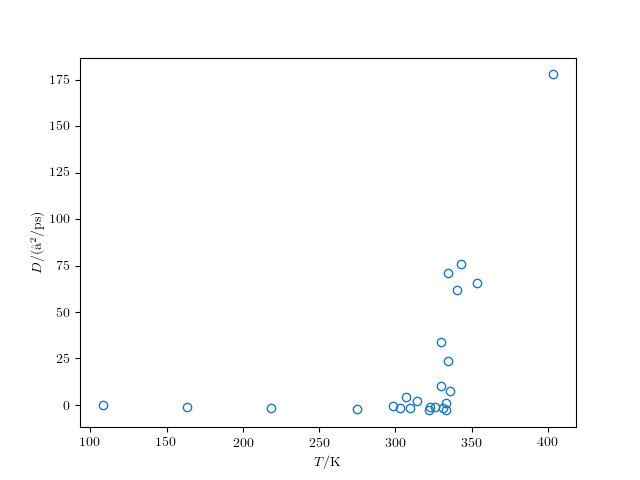
\includegraphics{melt.png}
		\caption{}
		\label{fig:melt}	
	\end{figure}

	\section{Introduction}
	
	
	\section{Theory}
	

	\section{Computational methods}
	
	\subsection{Scaling}

	
	
	
	\section{Implementation}

	
	\section{Analysis}
	
	\section{Conclusion}
	
	\printbibliography
	
	\appendix
	\section{Figures}
	

	
\end{document}